

\chapter{The mapping object}

%---------------------------------------------
%---------------------------------------------
%---------------------------------------------

\section{Introduction}

%---------------------------------------------
%\subsection{Target of mapping objects}

The mapping  are targeted to offer service for object that represent "smooth" mapping
from $\RR^n  \rightarrow  \RR^p$. As an exemple of class naturally derived from mappings used
in photogrammetry we have :

\begin{itemize}
	\item projection $\pi : (x,y,z) \rightarrow (i,j)$ function of an image sensor, as mapping $\RR^3 \rightarrow \RR^2$;

	\item extended projection $\pi_d :  (x,y,z) \leftrightarrow (i,j,d)$ , where $d$ is  the depth,
		as \emph{bijective} mapping of $\RR^3$  ( $\RR^3 \rightarrow  \RR^3$);

	\item distorsion of central perpective camera as  \emph{bijective} mapping of $\RR^2$;

	\item any  transformation  between two geodetic coordinate systems as \emph{bijective}  of  $\RR^3$.

\end{itemize}

The minimal service that a mapping must offer is to define the method $F$ that computes its values.
The kind of services that offers the  mappingi package is :

\begin{itemize}
     \item offer a default method computing the derivative $\frac{\partial F}{\partial x_i}$  using a basic finite differrence ,
           the class can override this default method if has something better to offer;

   \item for $\RR^n \rightarrow \RR^n$ compute the inverse $F^{-1}(v)$ of a given  value using  an iterative method;
           the class can override this default method if has something better to offer;

   \item compute the approximate inverse mapping  of given mapping using some basis of function and a  least square approach;

   \item offer an interface to use generated code of symbolic derivative as a mapping.
\end{itemize}

%---------------------------------------------
%---------------------------------------------
%---------------------------------------------

\section{General organization}

\subsection{Localization}

The declaration of class for mapping are localized in file {\tt include/MMVII\_Mappings.h}.

The definition of these class are located in folder {\tt src/Mappings/}.
As the mapping class are template, there is an explicit instantiation  for
all expected use.



%---------------------------------------------
\subsection{class {\tt cDataMapping}}

         %  -  -  -  -  -  -  -  -  -  -  -  -  -  -
\subsubsection{Templatization}
The base  class of all mappings is {\tt cDataMapping}, its a template class defined by $3$ 
parameters :

\begin{itemize}
    \item {\tt class Type} which is the floatting number type on which all the computation will be made,
          it can be {\tt tREAL4, tREAL8} or {\tt tREAL16} ;  practically it is for now obly used
          with {\tt tREAL8}; by the way some precaution where made to assure that
          the class be intantiated with any complete numeric type in case higher precision woul be required;


    \item {\tt const int DimIn} the dimension of input space;

    \item {\tt const int DimOut} the dimension of output space.
\end{itemize}

         %  -  -  -  -  -  -  -  -  -  -  -  -  -  -
\subsubsection{Values}

The fundamental method that a  mappings must define is  {\tt Value(s)} and it computes the values of 
the function.  Note that there exist two methods :

\begin{itemize}
     \item {\tt Value} that make the computation of single value ;

     \item {\tt Values} that make the computation of vector of values, it can  be used
           if the class has some parallelism option to accelerate the computation.
\end{itemize}

Note that these two virtual methods  have a default implementation : {\tt Value}
is implemented calling {\tt Values},  while {\tt Values} is implemented calling
{\tt Value}.  So obviously, an infinite recursion will occur if none is defined
(BTW it is dynamically detected in debug mode).  The interest being obviously that
in the derived class, it's possible to overload only one to benefit of both.

For {\tt Values} there are two options : 

\begin{itemize}
     \item  one option where the user gives the vector for storing the result;

     \item  one option where the class furnish its own buffer by reference,
            btw the same vector is always returned, so if the user memorize
            the adress, at next call it will be overwritten; so if the vector
            is not used immediately, a copy must be made.
\end{itemize}



         %  -  -  -  -  -  -  -  -  -  -  -  -  -  -
\subsubsection{Jacobian}

The jacobian is computed by returning pair point/Matrix  where point is
the value  and matrix is the  jacobian. This is because generaly when the 
user needs the jacobian he also needs the value, and also when you 
compute the jacobian, you have also computed the value .

Be aware that even if the user make a copy a vector containing results,
due to {\tt MMVII} implementation of matrix (using shared pointer on data),
at next call the jacobian will overwrite the previous call.  In this rare
case, user should call the {\tt Dup} method.

Like {\tt Value} the  class propose default definition of {\tt Jacobian} that user can override.
The users has three option :

\begin{itemize}
      \item  furnish at the construction of object a "small" value that will be used to 
	      compute the derivative by finite difference;  this small value is a point as  the
             meaning of "small" can be different in each dimension;

      \item  furnish a version that compute jacobian for a single point;

      \item  furnish a version that compute jacobian for a vector of  points;
\end{itemize}

We have the same behaviour that with value : version with point, if not overided, calls version
with vector \dots 

Note that using Jacobian, it is possible to compute the affine mapping that is the
differential in a given point. This is done with {\tt Linearize}  (BTW, currently
this is done in derivate class {\tt cDataNxNMapping}, probably to change).


%---------------------------------------------
\subsection{class {\tt cDataBoundedSet}}

This class is used  to represent bounded set of $\RR^n$. A bounded
set $S$ is made  from a box (that's why it is bounded) and a belong function $I$
(virtual method) such that :

\begin{itemize}
	\item if $I(p) >0$  then $p \in S $
	\item if $I(p) <0$  then $p \notin S $
	\item  ideally $I(p) =0$   then $p$ is at the frontier of $S$;
	\item  "ideally" $I$ should be the signed distance to the frontier or a continuous
		growing function of it (but it's not always possible);
\end{itemize}

Bounded set are used in particular in mapping inversion
by least-square to define the set on which inversion must be made. 
They are used also : for clipping a mesh, for computing z-bufer,
for defining the validity domain of a sensor  \dots list will probably grow.
The  different  {\tt cDataBoundedSet} existing now are :

\begin{itemize}
	\item  the box itself;
	\item  the box itself cliped by a sphere;
	\item  the image of a set $S$ by a mapping   $M$, which insideness is $I(M^{-1}(P))$;
	\item  $3d$ masks of {\tt MMV1} encapsulated as  {\tt cDataBoundedSet}.
\end{itemize}



%---------------------------------------------
%---------------------------------------------
%---------------------------------------------

\section{Simple predefinite mappings}


%---------------------------------------------
\subsection{class {\tt cMappingIdentity}}

Sometime it can be usefull to desribe the identity function as a mapping.
For example as an estimation of rough inverse in iterative inversion.

%---------------------------------------------

\subsection{class {\tt cIMElemLinear}}
\subsection{class {\tt cBijAffMapElem}}
\subsection{class {\tt cInvertMappingFromElem}}

%---------------------------------------------
%---------------------------------------------
%---------------------------------------------

\section{Mapping inversion}

\subsection{Class {\tt cDataNxNMapping}}

This class is just a specializion for case where {\tt DimIn==DimOut}. All stuff
related to inversion will inherit from this class.


\subsection{Class {\tt cDataInvertibleMapping}}

This class is the mother class of mapping that are invertible. An invertible
mapping must simply define {\tt Inverse}  or {\tt Inverses} method that compute
the inverse of {\tt Value}.  Like usual, by default {\tt Inverse} calls  {\tt Inverses}
and {\tt Inverses} calls  {\tt Inverse}; so one at least must be defined else an
inifinite recursion will occur.


\subsection{Class {\tt cDataInvertOfMapping}}

When we have a mapping $M$ that is invertible, this class create a mapping $M'$
that contain a pointer on $M$ and such hat  $M'.Val(P) = M.Inv(P)$ and $M'.Inv(P) = M.Val(P)$


\subsection{Class {\tt cDataIterInvertMapping}}

This is here that we begin to really do something \dots

This class offer a concrete computation of the inverse function by iterative gradient method .
Given $Y$, we want to find $X$  such that $F(X)=Y$,  if we have a current "estimation" $X_k$,
we write $F(X_{k+1}) = F(X_k) + \nabla (X_{k+1}-X_k) = Y$ then :

\begin{equation}
	X_{k+1} = X_k + \nabla ^{-1} (Y-F(X_k)) \label{IterGradInv}
\end{equation}

The method starts  from an initial "guess" $X_0$ and iterates equation~\ref{IterGradInv} until some
condition linked to thresholds $\epsilon,N_{iter}$ is reached ($|F(X_k)-Y|<\epsilon$ or $k>N_{iter}$).
This iterative schema require an initialization $X_0$, this is why the constructor take as
argument a mapping named {\tt RoughInv}. For the rough inverse sometime the user
will have information to give a good estimation , in other case identity (or even 
null function) can works well is the mapping is close to a linear form.  For more difficult case,
a convenient solution can be to use the facilities {\tt cComputeMapInverse} describes in~\ref{CompMapInv}
that compute approximate inverse by least square on a given basis of function (it's the method
used for invering distorsion).

\subsection{Class {\tt cDataIIMFromMap}}

This class is just an adaptator to use iterative inversion . Suppose class {\tt cMapSth} exist,
you want to invert it by iterative scheme of  {\tt cDataInvertOfMapping}, but if you cannot
modify {\tt cMapSth}, you cannot make it inherit of {\tt cDataInvertOfMapping}. So you can
use {\tt cDataIIMFromMap}, that owns a pointer on {\tt cMapSth} on inherit of {\tt cDataIterInvertMapping}
to make the inversion.

%---------------------------------------------
%---------------------------------------------
%---------------------------------------------

\section{Least square fitting, and use for inversion}

\section{class {\tt cLeastSqComputeMaps}}

This pure virtual  class can be used to estimate a mapping by least square from a set of samples.
Its most current used, will probably be for estimation of inverse function from direct.
Suppose we have a set of function  $F_1 \dots F_M$ with  $ F_k : \RR^n  \rightarrow  \RR^p$.
We want to estimate $F$ as a linear combination :

\begin{equation}
	F = \sum  a_k  F_k \label{EqMapLsq1}
\end{equation}

We have a set a point $P_1 \dots P_L $ for which we know  the value $Q_l$ such
that $F(P_l) = Q_l$,  then we solve by least square equation~\ref{EqMapLsq2} :

\begin{equation}
	Q_l = \sum  a_k  F_k(P_l)  \label{EqMapLsq2}
\end{equation}

In class  {\tt cLeastSqComputeMaps} there is not explicit description of $F_k$,
instead this is the pure virtual method {\tt ComputeValFuncsBase}, to override,
that must return for a given point $P$ the vector $F_1(P) \dots F_M(P)$.

The method {\tt AddObs(P,Q)}, and its variants, add an equation corresponding to 
equation~\ref{EqMapLsq2}

%---------------------------------------------
\section{class {\tt cComputeMapInverse}}

\label{CompMapInv}

This class use a well known method for computing apprixomate inverse, if
we can compute direct value of $M$, and have a basis $F_1 \dots $
of function for $M^{-1}$, we just have to generate sufficient sample $P_l$
to solve by least square :


\begin{equation}
	P_l =  M^{-1}(M(P_l)) = \sum  a_k  F_k(M(P_l))  \label{EqMapLsq3}
\end{equation}
 
Given a certain maping $M$, a certain basis of function $F_k$ and least square system
described by {\tt cLeastSqComputeMaps}, solving equation~\ref{EqMapLsq3}, is
quite obvious \emph{except} for one issue : how do we generate the $P_l$.
{\tt cComputeMapInverse} offers a solution that is expected to  satisfy most
current case and be easy to use.  The counterpart is that the implementation
is not trivial, so we give some detailed explanation of the algorithm for future maintenance.
The method has been thought specifically to be used in approximate inversion of distorsion.

The first set of parameter the user must specify :

\begin{itemize}
    \item obviously  mapping to inverse $M$ must be furnish, we will call $M'$ the pseudo
          inverse to compute that will satisfy $M'(M(P)) \simeq P$ for all samples we will generate;


    \item the domain $D'$ on which inversion will have to be made, remember we 
          are computing the pseudo inverse, and we cannot expect $M' \circ M = Id$
          on $\RR^n$, so we have to fix domain on which equation~\ref{EqMapLsq3}
          is optimized;

          note that the domain is specified in ouptut coordinates : a point is
          to be selected if $M(P) \in D'$;  it's not sure if this convention we always
          be the best one, at least its convenient for distorsion because the domain
          we want to specify  is  the sensor rectangle (or circle for fish-eye);

    \item  a seed point $P_0$ that is supposed to belong to $D'$  $M(P_0) \in D$;

    \item  a step $S$ for generating a regular greed in input coordinates;

    \item  a threshold $TJ$ on regularity, $TJ<1$, the use of this threshold is to assure
           that the $M$ is bijective on the domain where we do the computation;
           let $J_0$  be the jacobian in $P_0$, we will consider only point $P$
           where the jacobian $J(P)$ is sufficienlty close to $J_0$

\end{itemize}

\begin{equation}
    ||  J(P) J_0^{-1} -Id|| < TJ  \label{EqJacCloseJ0}
\end{equation}


To compute the points,  on a regular grid, we first need to have a majoration
of the box of interest in input coordinate, because we will need to compute an
image to mark the point of this grid . The domain $D$ is a boundet set,
so it is contained in a box $B$, and we use $J_0^{-1}(B)$ as a first estimation,
however as we want to be sure not to omit any point we dilate it by a factor
$\frac{1}{1-TJ}$.




\begin{figure}
\centering
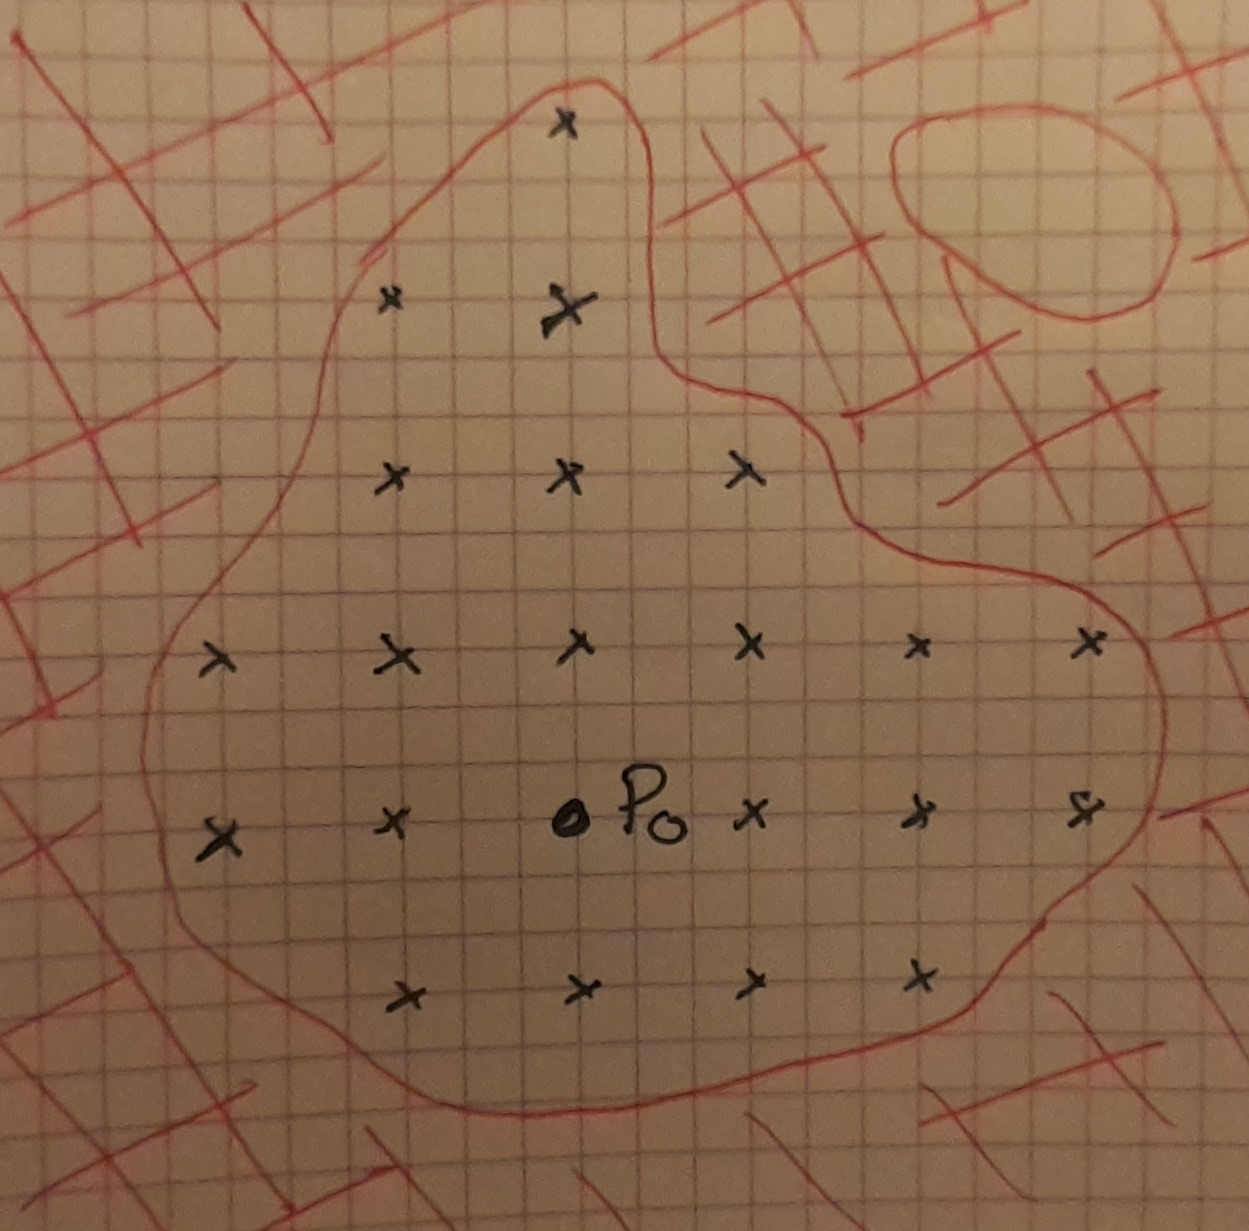
\includegraphics[width=6cm]{Programmer/ImagesProg/PointInver-Interior.jpg}
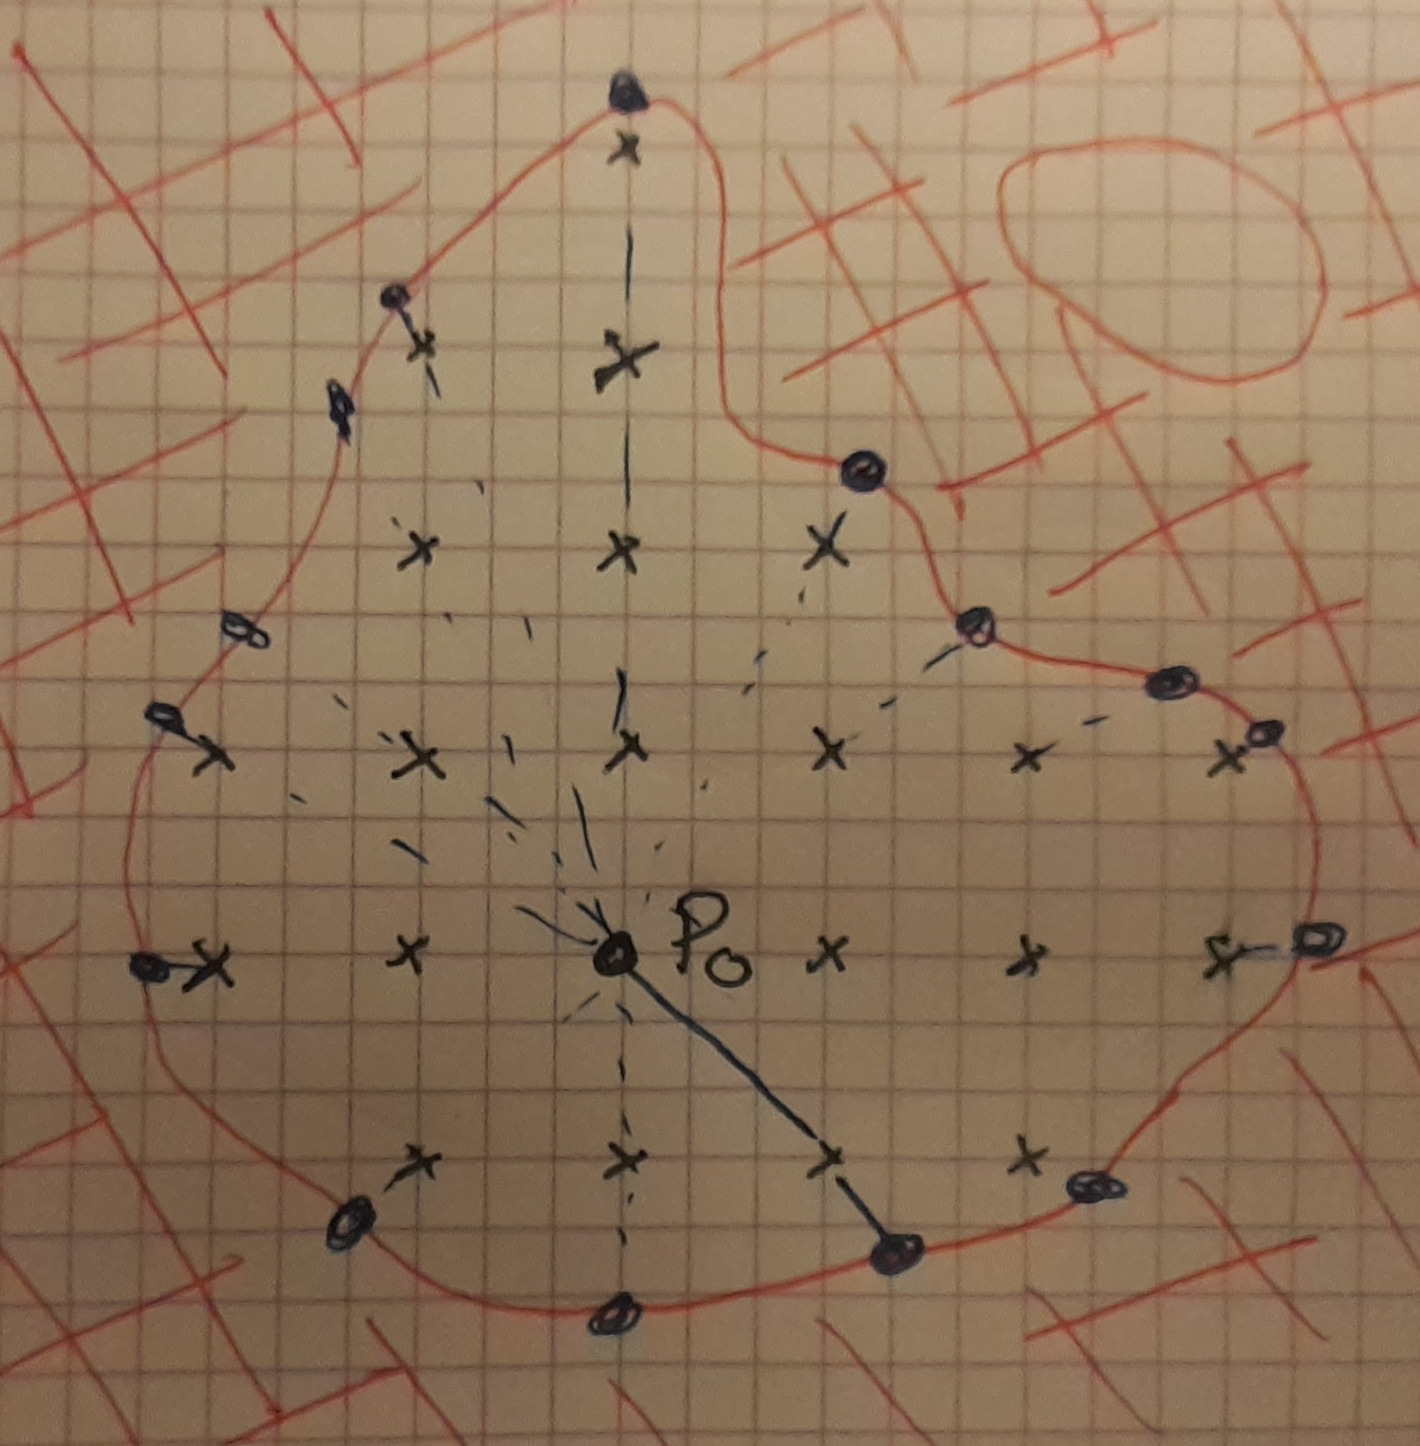
\includegraphics[width=6cm]{Programmer/ImagesProg/PointInver-WFront.jpg}
\caption{Generation of sample point for inversion : interior only (left) and with frontier(right)}
\label{fig:PointInvGen}
\end{figure}


Once we have the image, we make a first computation of the "interior" points,
we start from the singleton containing the seed $\{P_0\}$ and compute the connected 
components by iteratively adding the neighboor $P$ respecting equation~\ref{EqJacCloseJ0}
and  $M(P) \in D'$.  This lead to a first set as illustrated by left image 
of figure~\ref{fig:PointInvGen}.

However, this may not be sufficient as we "know" that if computation of such function
is relatively good in interpolation, it can be very unacurate in extrapolation. So there
is a risk that the estimation may be unaccurate close to the frontier; a solution
could be to have a very small step in the grid generation, but this could lead to
a heavy computation.  To overcome this difficulty, we proceed this way :

\begin{itemize}
    \item we select all computed the point on the grid that are that the frontier
          (those who are in $D'$ and  have a neihgboor not belonging to $D'$);

    \item  for each such point $P$,  we use a dicothomic algorithm to prolongate the
	   line $P_0P$ with a point in $D'$ and as close as possible to a point out $D'$,
           this is illustrated by right image of figure~\ref{fig:PointInvGen}.
\end{itemize}


%---------------------------------------------
%---------------------------------------------
%---------------------------------------------

\section{Symbolic derivative \& mappings}

It's often convenient to encapsulate generated code in the class
mappings that offer a higher level description of the same code. 
It's for now the most current case of using mappings.


\subsection{class {\tt cDataMapCalcSymbDer}}

This class embeds two {\tt cCalculator}, one {\tt CVal} for computing
the values, and one {\tt CDer} for computing values and derivatives,
and use them for returning {\tt Values} and {\tt Jacobian}.

There is few restriction on  {\tt CVal} and {\tt CDer}, except that
the number of unkowns is equal to {\tt DimIn} and number of value
returned is equal to {\tt DimOut}.


\subsection{class {\tt cDataNxNMapCalcSymbDer}}

Create a specialization for the case {\tt DimIn == DimOut}.


\subsection{class {\tt cLeastSqCompMapCalcSymb}}

This class use a {\tt cCalculator} for describing a basis of function
that can be used to approximate a funtion (or often its inverse) by least square.

To make it concrete, we anticipate and use the case of basic distorsion, that will be re-explained in 
more detail and more general model in the following chapters. 
Consider a basic model of radial distorsion that integrate a radial distorsion, with
coefficient $k_1,k_2$ and a linear distortion parametrize by $b_1,b_2$. It correspond
to equation~\ref{BasicDist4P}:

\begin{equation}
	D(x,y) =  
	       (1 + k_1 \rho ^2  + k_2  \rho^4)  \begin{pmatrix} x \\ y \end{pmatrix}
	      +   \begin{pmatrix} b_1 x + b_2 y  \\  0 \end{pmatrix}
	\label{BasicDist4P}
\end{equation}

The calculator associated to $D$ will return a formula similar to equation~\ref{BasicDist4P}.
Now we want to compute a pseudo-inverse of $D$, the choice of the basis function will be
a compromise between  the accuracy and the efficiency; basically for accuracy, the more
function the better as long as we avoid degenerency by over-parametrization.
Admit  we make the following reasonnable choice for the basis function  :

\begin{itemize}
    \item  for the radial part, which is generally the most significant,  we need to be accurate;
              also  we take into account the fact that te inverse of a radial function is a radial
              function; in this examplae we take  a radial invers with  $3$ coefficient
              (it's arbitrary, and $2$ or $4$ may be also a good choice, to adapt with the context);

    \item   for the linear part, wich is generally "small", the can restrict ourself to
	    the Taylor expansion $(Id+\epsilon)^1 = Id-\epsilon$, so the functionnal space
            for the inverse is the same that the direct space;
\end{itemize}

So concretely in this example, the functionnal space pseudo invers $D'$  could be given by  :

\begin{equation}
	D'(x,y) =  
	       (1 + k_1 \rho ^2  + k_2  \rho^4 + k_3 \rho^6)  \begin{pmatrix} x \\ y \end{pmatrix}
	      +   \begin{pmatrix} b_1 x + b_2 y  \\  0 \end{pmatrix}
	\label{BasicDistInv5P}
\end{equation}

However , for {\tt MMVII} to be able to separate each of $5$ function  that constitute the basis
of this functionnal space,   $D'$ must not be describe as a sum, conversely we must describe separately
the $10$ coordinate function ($5$ functions of $x,y$) that  constitute the base :

\begin{equation}
	\begin{pmatrix} x \rho ^2 & x \rho ^4  &  x \rho ^6   & x & y \\ 
		        y \rho ^2 & y \rho ^4  &  y \rho ^6   & 0 & 0
       \end{pmatrix}
       =
	\begin{pmatrix} f^1_x &  \dots  & f^5_x  \\
		        f^1_y &  \dots  & f^5_y
       \end{pmatrix}
\end{equation}

In this example, the  {\tt cCalculator} will have to  return  $10$ coordinates as a
vector:
\begin{equation}
    [ f^1_x,  \dots  , f^5_x , f^1_y , \dots, f^5_y]   \label{Vec10Dist}
\end{equation}

Finally, what the class  {\tt cLeastSqCompMapCalcSymb} really does, is takes a
calculator than return a vector similar to~\ref{Vec10Dist} and use it to override
the method {\tt ComputeValFuncsBase}.



